%%%%%%%%%%%%%%%%%%%%%%%%%%%%%%%%%%%%%%%%%%%%
\section{air4children}


\begin{frame}
      \frametitle{Table of Contents}
      \tableofcontents[currentsection]
\end{frame}


%%%%%%%%%%%%%%%%%%%%%%%%%%%%%%%%%%%%%%%%%%%%%
\subsection{Open source software and hardware in AI and Robotics}

%%%%%%%%%%%%%%%%%%%%%%%%%%%%%%%%%%%%%%%%%%%%%%%%%%%%%%%%
{
%\paper{Savage N. 2021 in Nature}
\begin{frame}{Open source software and hardware in AI and Robotics}

      \begin{figure}
        \centering
        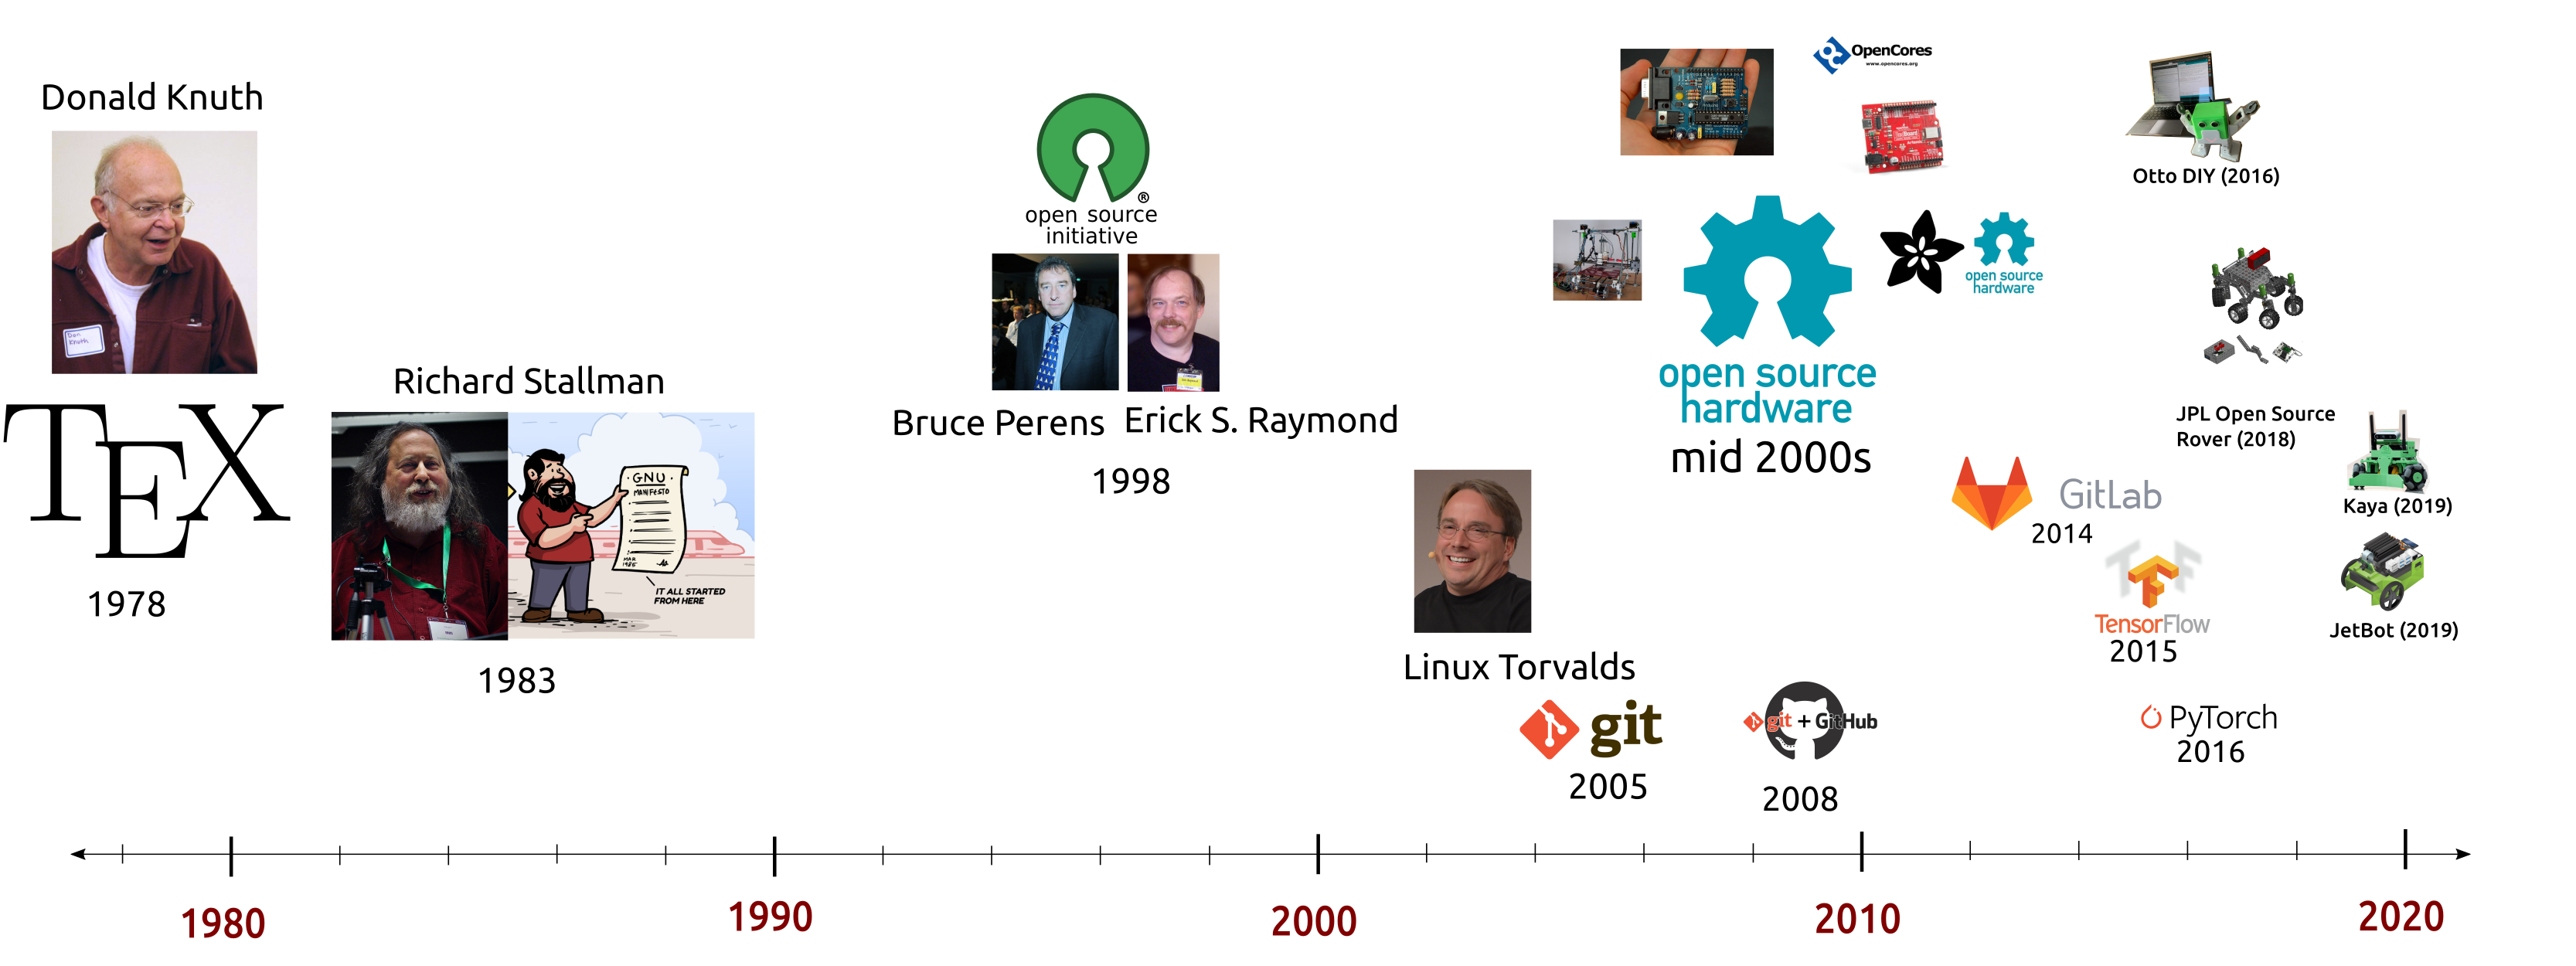
\includegraphics[width=1.0\textwidth]{./figures/timeline-osh/outputs/drawing-v00.png}
        %\caption{}
      \end{figure}
\end{frame}
}

%%%%%%%%%%%%%%%%%%%%%%%%%%%%%%%%%%%%%%%%%%%%%%%%%%%%%%%%
{
%\paper{Lastname N. YEAR in journal of...}
\begin{frame}{
air4children, Artificial Intelligence and Robotics for Children
}
 
  \begin{columns}
  \begin{column}{.7\linewidth}

  \begin{itemize}
    \item create a more inclusive, affordable and fair participation of children in AI and Robotics,
    \item create child-centred AI and Robotics curriculums based on Montessori Education, and
    \item build Open source robots to be affordable and fun. 
  \end{itemize}

    \end{column}


  \begin{column}{.4\linewidth}

      \begin{figure}
        \centering
        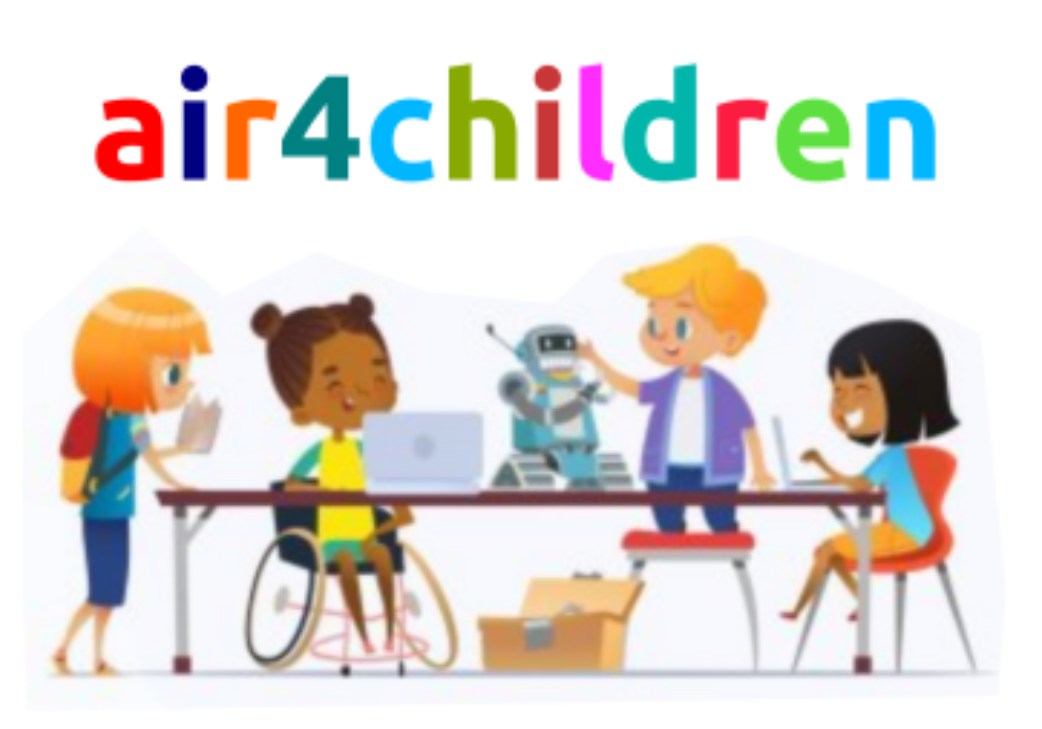
\includegraphics[width=0.95\textwidth]{./figures/logo/outputs/drawing-v00.png}
      \end{figure}

    \end{column}
  \end{columns}

\end{frame}
}




%%%%%%%%%%%%%%%%%%%%%%%%%%%%%%%%%%%%%%%%%%%%%
\subsection{Prototyping and piloting Open Source Robots}

%%%%%%%%%%%%%%%%%%%%%%%%%%%%%%%%%%%%%%%%%%%%%%%%%%%%%%%%
{
\paper{Xochicale M. 2014, \it{Proposal of Libre Robotics} }
\begin{frame}{Prototyping Open Source Robots (2013 -- 2017)}
      \begin{figure}
        \centering
        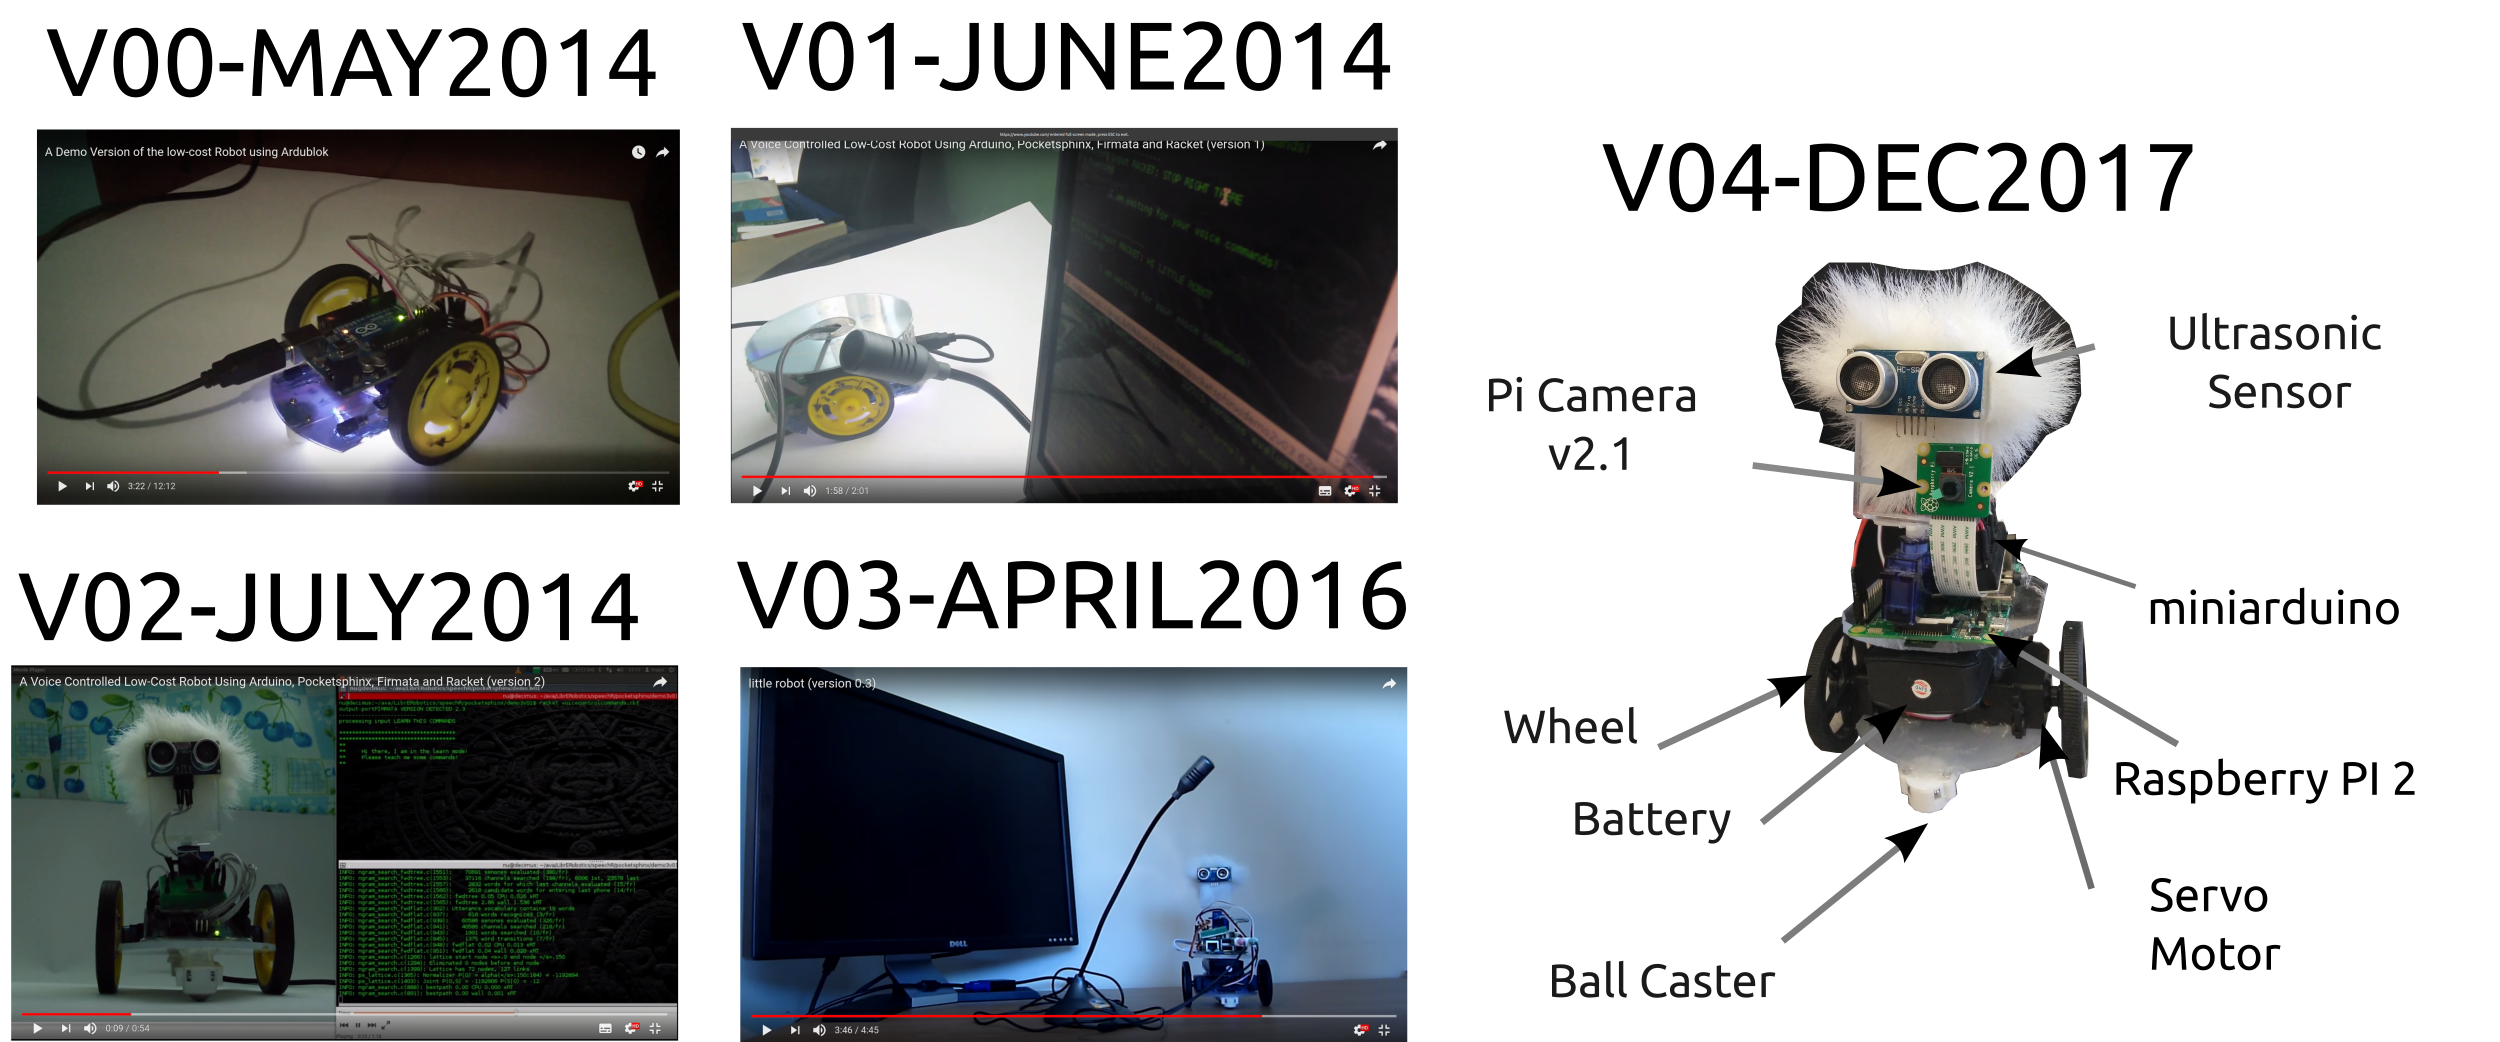
\includegraphics[width=1.0\textwidth]{./figures/air4children-a/outputs/drawing-v00.png}
        %\caption{}
      \end{figure}
\end{frame}
}

%%%%%%%%%%%%%%%%%%%%%%%%%%%%%%%%%%%%%%%%%%%%%%%%%%%%%%%%
{
\paper{Xochicale M. 2015 in Mecate; Parra C. et al. 2016, \it{Otto DIY}}
\begin{frame}{Piloting robot prototypes (2015 -- 2019)}
      \begin{figure}
        \centering
        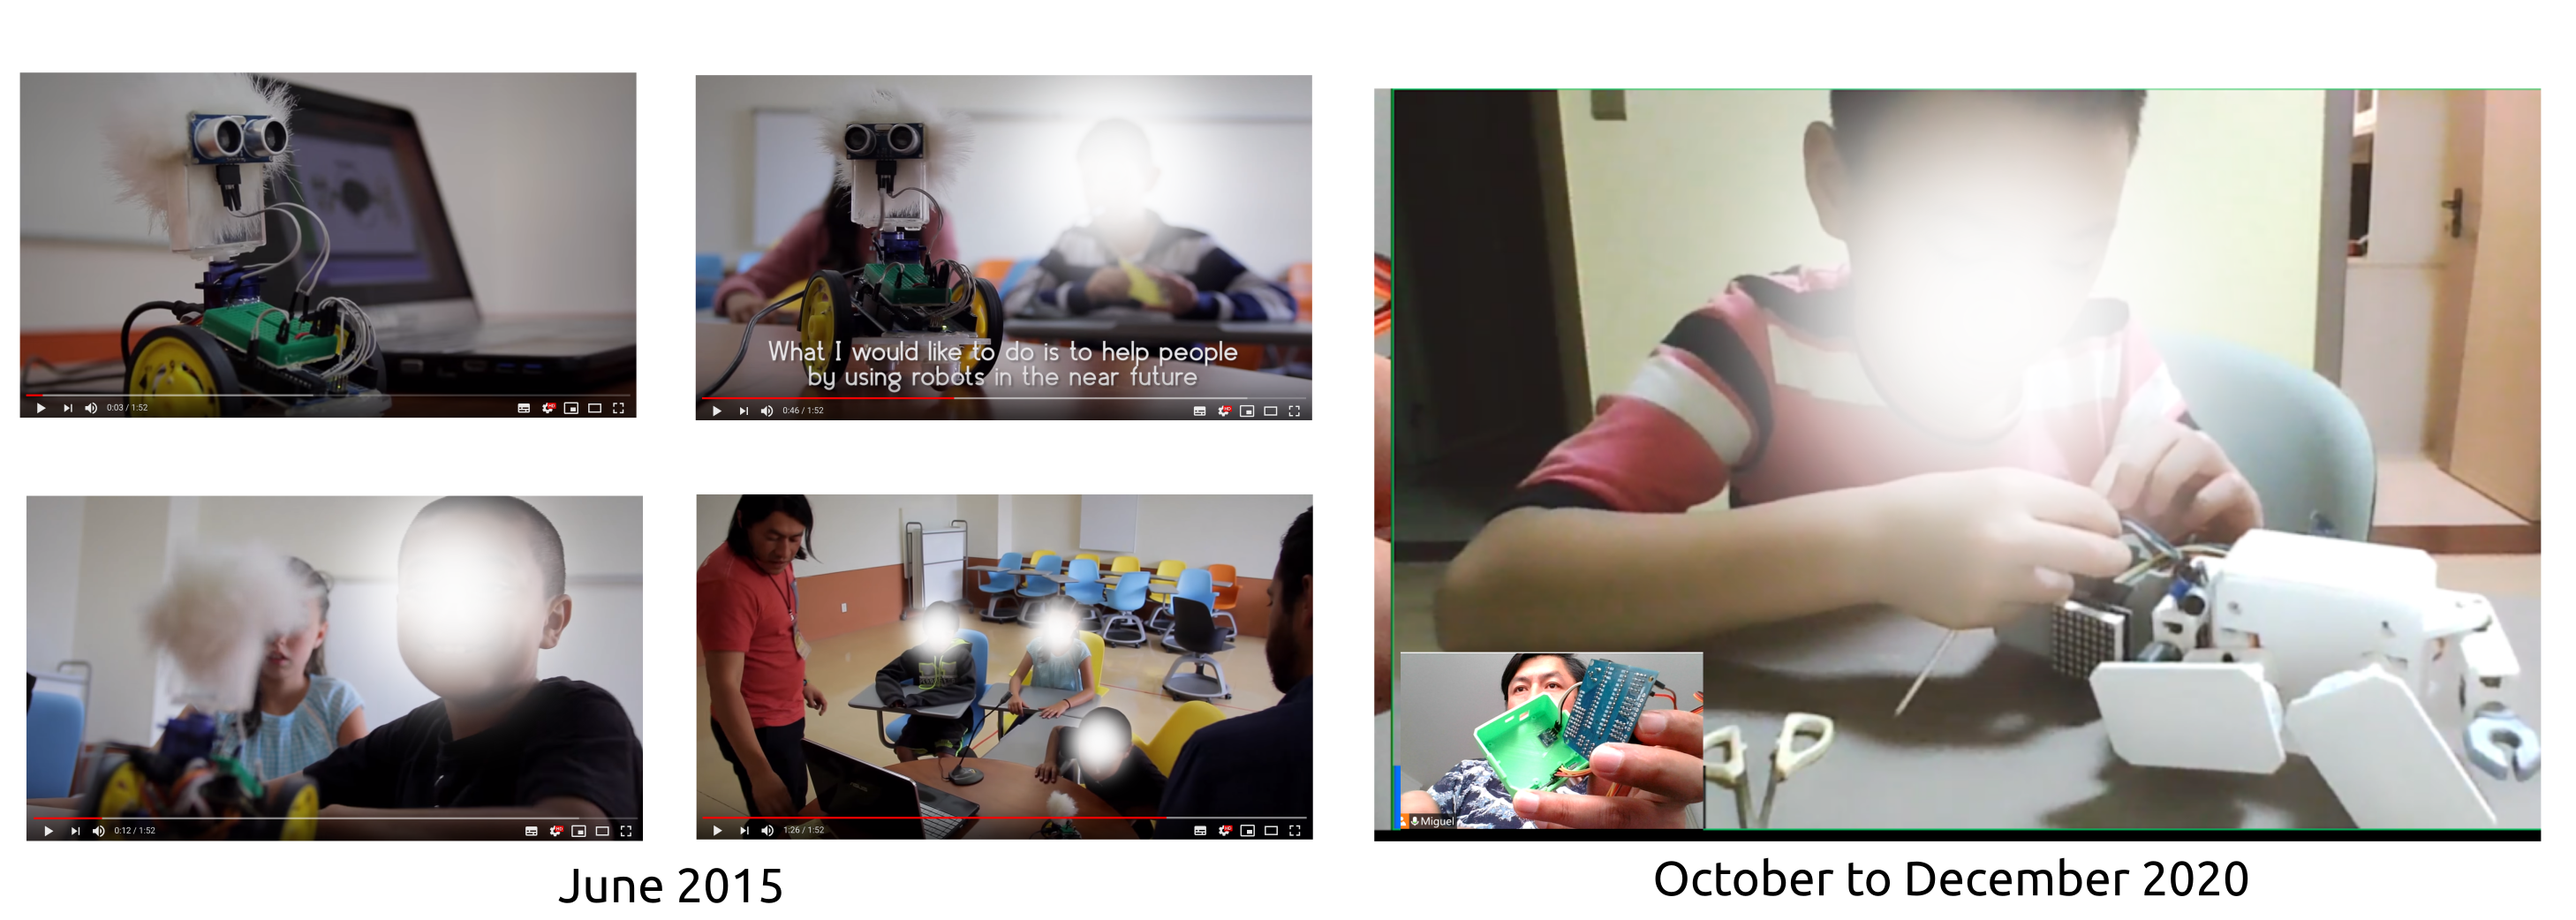
\includegraphics[width=1.0\textwidth]{./figures/air4children-b/outputs/drawing-v00.png}
        %\caption{}
      \end{figure}
\end{frame}
}

%%%%%%%%%%%%%%%%%%%%%%%%%%%%%%%%%%%%%%%%%%%%%
\subsection{Montessori Education}

%%%%%%%%%%%%%%%%%%%%%%%%%%%%%%%%%%%%%%%%%%%%%%%%%%%%%%%%
{
\paper{Elkin M., Sullivan A, Bers 2014 in Journal of Information and Technology}
\begin{frame}{Montessori Education} 
\vspace{3mm}
%\it{
"The hand is the instrument of the mind."
%} 
%\\
Dr. Maria Montessori (1970-1952).

\vspace{2mm}
    \begin{figure}
        \centering
        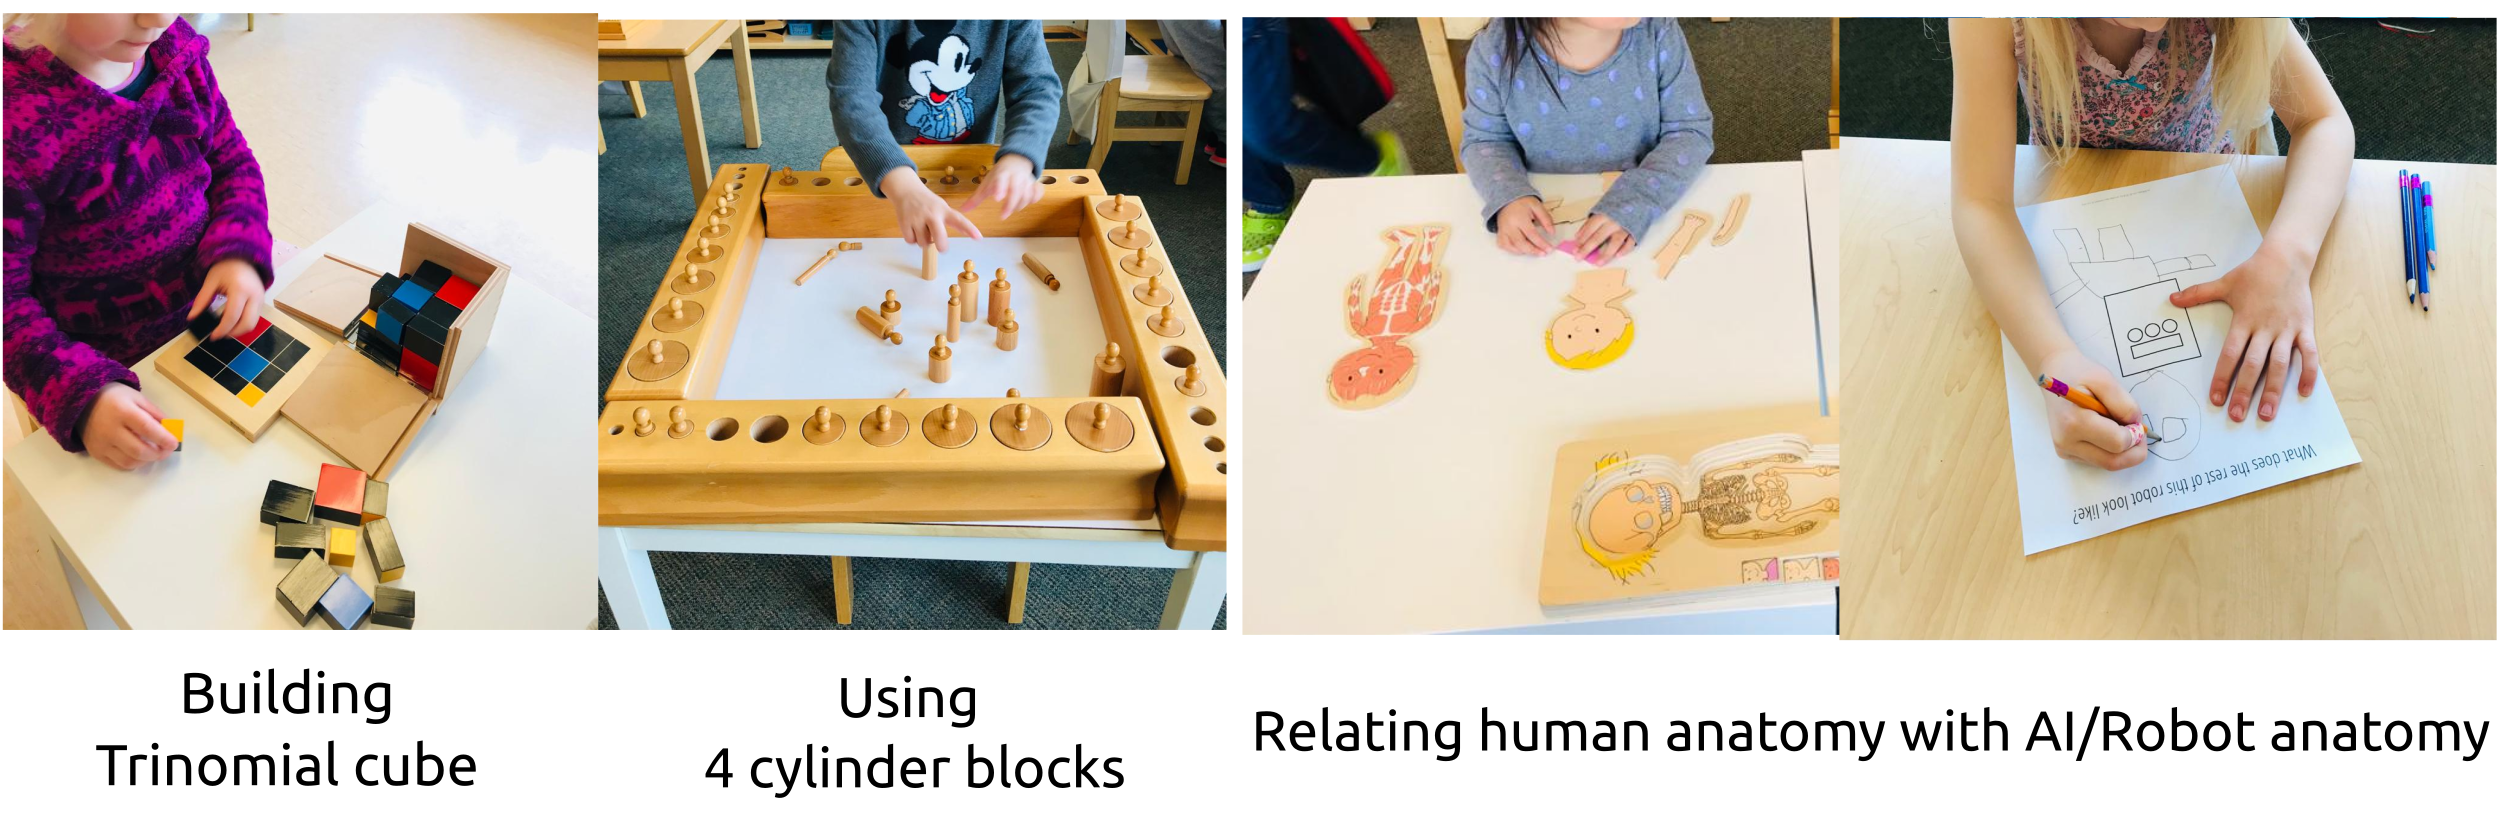
\includegraphics[width=1.0\textwidth]{./figures/montessori/outputs/drawing-v00.png}
        %\caption{}
      \end{figure}

Children are participating in creative explorations to develop fine motor skills and to engage in collaborative and teamwork activities. 

\end{frame}
}



%%%%%%%%%%%%%%%%%%%%%%%%%%%%%%%%%%%%%%%%%%%%%%%%%%%%%%%%
{
\paper{Mohammad T. et al., 2017; Harden R. M. 1999 in Journal of Medical Teacher}
\begin{frame}{Spiral Learning Method}

  \begin{figure}
        \centering
        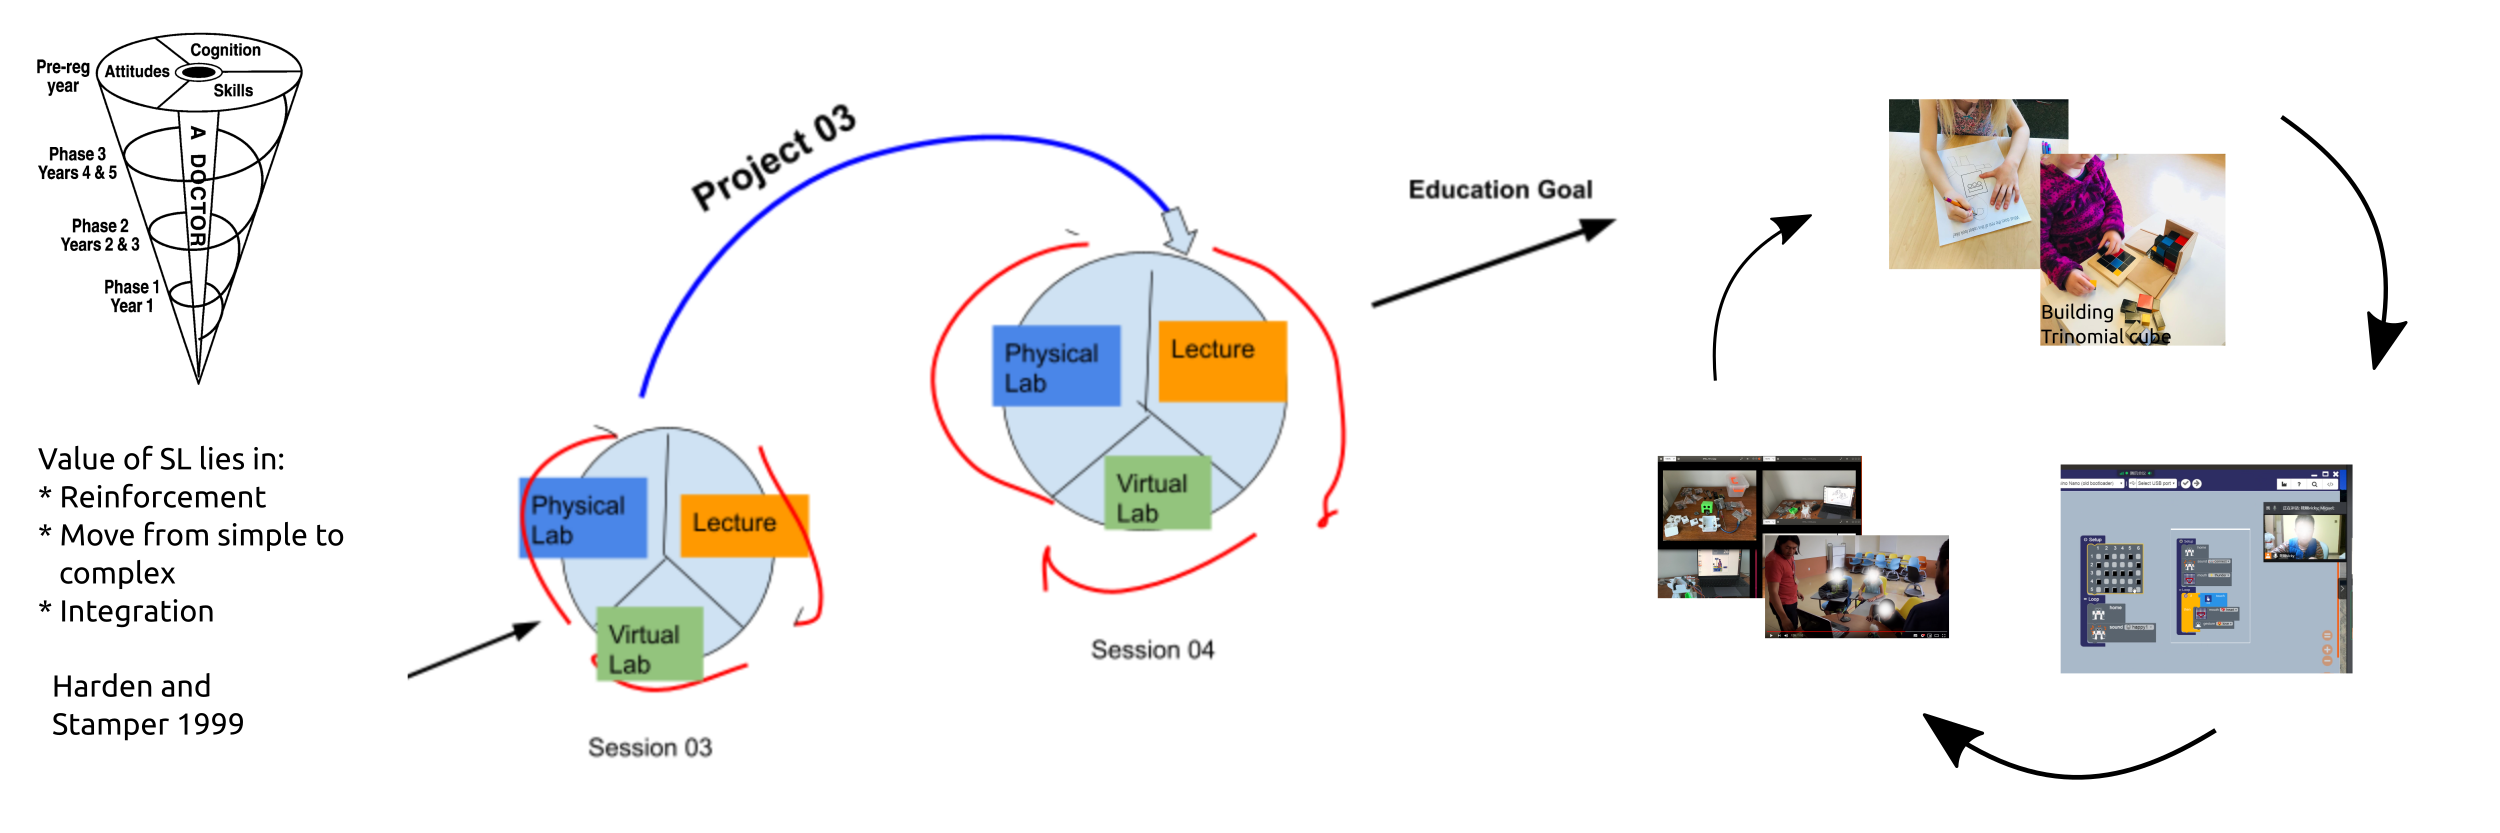
\includegraphics[width=1.0\textwidth]{./figures/teaching-materials/outputs/drawing-v02.png}
        %\caption{}
      \end{figure}
\end{frame}
}
